\documentclass{beamer}
\beamertemplatenavigationsymbolsempty
\usepackage{amsmath, amssymb, hyperref, graphics}
\usepackage{tikz}
%\usepackage{mathpazo}
\usetikzlibrary{graphs}
\usetikzlibrary{graphs.standard}


\newcommand{\Z}{\mathbb{Z}}
\newcommand{\Q}{\mathbb{Q}}
\newcommand{\R}{\mathbb{R}}


\title{Graph Theory Lecture 3}

\begin{document}
\begin{frame}{Which graphs are/aren't isomorphic?  Prove it.}
  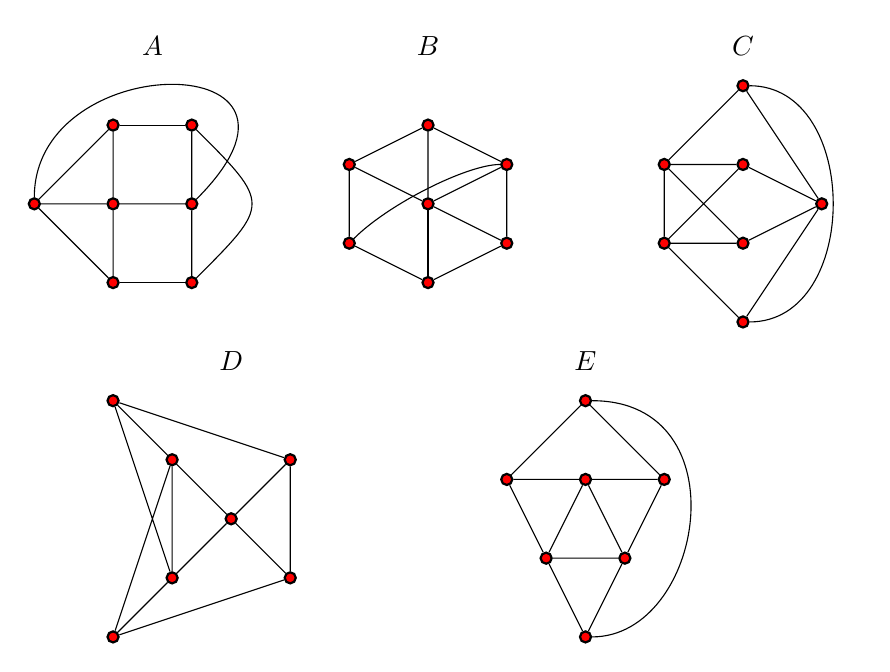
\begin{tikzpicture}
\node at (1.5,2) {$A$};
\node at (5,2) {$B$};
\node at (9,2) {$C$};
\node at (2.5, -2) {$D$};
\node at (7, -2) {$E$};
  \begin{scope}[every node/.style={circle, draw, fill=red, inner sep=0pt, minimum width=4pt, thick}]

    
  \node (a) at (0,0) {};
  \node (b) at (1,1) {};
  \node (c) at (1,0) {};
  \node (d) at (1,-1)  {};
  \node (e) at (2,1) {};
  \node (f) at (2,0) {};
  \node (g) at (2,-1) {};

  \draw (a) -- (b) -- (c) -- (d) -- (a) -- (c) -- (f) -- (e) .. controls (3,0) and (3,0) .. (g)--(f) .. controls (4,2) and (0,2) .. (a);
  \draw (b)--(e);
  \draw (d)--(g);
  

  \begin{scope}[xshift=4cm, scale=.5]
  \node (a) at (0,1) {};
  \node (b) at (0,-1) {};
  \node (c) at (2,2) {};
  \node (d) at (2,0)  {};
  \node (e) at (2,-2) {};
  \node (f) at (4,1) {};
  \node (g) at (4,-1) {};

\draw (b)--(a)--(c)--(f)--(g)--(e)--(b) .. controls (1,0) and (3,1) .. (f)--(d)--(g);
\draw (a)--(d)--(c);
\draw (d)--(e);

    \end{scope}
  
  \begin{scope}[xshift=8cm, scale=.5]
  \node (a) at (0,1) {};
  \node (b) at (0,-1) {};
  \node (c) at (2,3) {};
  \node (d) at (2,1)  {};
  \node (e) at (2,-1) {};
  \node (f) at (2,-3) {};
  \node (g) at (4,0) {};

  \draw (a)--(c) .. controls (5,3) and (5, -3) .. (f)--(b)--(a)--(d)--(b)--(e)--(a);
  \draw (c)--(g)--(d);
  \draw (e)--(g)--(f);

    \end{scope}

  \begin{scope}[yshift=-4cm, xshift=1cm, scale=.75]
  \node (a) at (0,2) {};
  \node (b) at (0,-2) {};
  \node (c) at (3,1) {};
  \node (d) at (3,-1)  {};
  \node (e) at (1,1) {};
  \node (f) at (1,-1) {};
  \node (g) at (2,0) {};

  \draw(a)--(c)--(d)--(b)--(e)--(a)--(f)--(e)--(g)--(c);
  \draw (g)--(d);
  \draw (b)--(f)--(g);
  
    \end{scope}

  \begin{scope}[yshift=-4cm, xshift=6cm, scale=.5]
  \node (a) at (2,3) {};
  \node (b) at (0,1) {};
  \node (c) at (2,1) {};
  \node (d) at (4,1)  {};
  \node (e) at (1,-1) {};
  \node (f) at (3,-1) {};
  \node (g) at (2,-3) {};


  \draw (a)--(b)--(c)--(d)--(a) .. controls (6,3) and (5, -3) .. (g)--(f)--(e)--(g);
  \draw (b)--(e)--(c)--(f)--(d);
    \end{scope}  
\end{scope}

  
\end{tikzpicture}  

  

\end{frame}

\begin{frame}{One solution to warm-up}
  \begin{itemize}
  \item Graph $B$ has a vertex of degree 5; others have degree sequence $[4,4,4,3,3,3,3]$, so none are isomorphic to $B$.
  \item In $A, D, E$, the three vertices of degree 4 all touch, but not in $C$, so none are isomorphic to $C$.
  \item In $A, D$, every vertex is adjacent to a vertex of degree 4, but not in $E$, so none are isomorphic to $E$.   
  \item But we see below $A$ is isomorphic to $D$:
  \end{itemize}
\begin{center}
  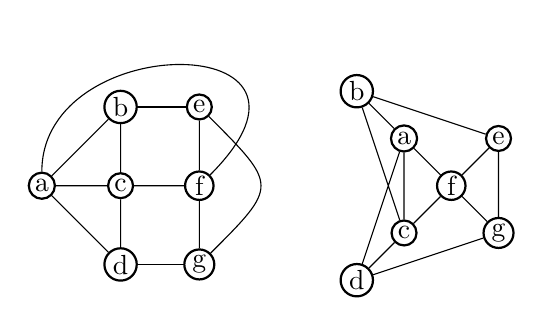
\begin{tikzpicture}[every node/.style={circle, draw, thick, inner sep=1pt}]
  \node (a) at (0,0) {a};
  \node (b) at (1,1) {b};
  \node (c) at (1,0) {c};
  \node (d) at (1,-1)  {d};
  \node (e) at (2,1) {e};
  \node (f) at (2,0) {f};
  \node (g) at (2,-1) {g};

  \draw (a) -- (b) -- (c) -- (d) -- (a) -- (c) -- (f) -- (e) .. controls (3,0) and (3,0) .. (g)--(f) .. controls (4,2) and (0,2) .. (a);
  \draw (b)--(e);
  \draw (d)--(g);

  \begin{scope}[xshift=4cm, scale=.6]
  \node (a) at (0,2) {b};
  \node (b) at (0,-2) {d};
  \node (c) at (3,1) {e};
  \node (d) at (3,-1)  {g};
  \node (e) at (1,1) {a};
  \node (f) at (1,-1) {c};
  \node (g) at (2,0) {f};

  \draw(a)--(c)--(d)--(b)--(e)--(a)--(f)--(e)--(g)--(c);
  \draw (g)--(d);
  \draw (b)--(f)--(g);
  
    \end{scope}
\end{tikzpicture}
\end{center}
  
\end{frame}



\begin{frame}{A forest is a bunch of trees}
  \begin{figure}
            \includegraphics[width=\textwidth]{Pictures/forest.png}
\caption{A forest of three trees}
  \end{figure}

  \begin{definition}\begin{itemize}
    \item A \emph{forest} is a graph without cycles
    \item A \emph{tree} is a connected graph without cycles
    \end{itemize}
  \end{definition}
\end{frame}

\begin{frame}{The Treachery of Definitions (After Magritte)}
  \begin{figure}
    \includegraphics[width=.85\textwidth]{Pictures/NotATree.jpg}
    \caption{Ceci n'est pas un arbre  (This is not a tree)} 
\end{figure}
\end{frame}

\begin{frame}{$\lfloor 13/2\rfloor$ ways of looking a tree (After Wallace Stevens)}
  \begin{block}{Proposition:} Let $G$ be a graph with $n$ vertices.  The following are equivalent.
    \begin{enumerate}
    \item $G$ is a tree (i.e., $G$ connected but has no cycles)
    \item There is a unique path in $G$ between any two vertices
    \item $G$ is connected and has $n-1$ edges
    \item $G$ has no cycles and has $n-1$ edges
    \item $G$ is connected, but removing any edge disconnects $G$
    \item $G$ has no cycles, but adding any edge creates a cycle
      \end{enumerate}
  \end{block}
  \begin{block}{Informally: Trees are Goldilocks graphs}
    \begin{itemize}
\item    Trees have enough edges: they're connected \\
\item    Trees don't have too many edges: they have no cycles
  \end{itemize}
\end{block}

\end{frame}

\begin{frame}{Make like a tree and get out of here (After Biff Tannen)}

  \begin{definition}[Tree]Let $T$ be a tree.  A vertex $v\in T$ is a \emph{leaf} if it has degree 1.\end{definition}
\begin{lemma}Let $T$ be a tree with $2\leq n<\infty$ vertices.  Then $T$ has at least two leaves. \end{lemma}

\begin{block}{Proof 1: See title of slide.}
Pick an edge, and try to ``leave'' -- that is, walk as far as you can.
  \begin{itemize}
  \item No loops, so you'll never return to where you are
  \item Finitely many vertices, so it can't go on forever
  \end{itemize}
Eventually you'll get stuck -- that's a leaf.
\end{block}
\end{frame}
\begin{frame}{Pruning Trees}
  \begin{block}{Part of Proposition:} If $T$ is a tree with $n$ vertices, then $T$ has $n-1$ edges.
  \end{block}
  \begin{block}{Proof: Induct on $n$}
    \begin{itemize} \item Base case: $n=1$
      \item Now assume that all trees with $n-1$ vertices have $n-2$ edges
      \item If $T$ is a tree with $n$ vertices, it has a leaf $v$ (by Lemma)
        \item Delete $v$ and the edge next to it to get a new tree $T^\prime$ 
        \item $T^\prime$ has $n-1$ vertices, so $n-2$ edges, so $T$ has $n-1$ edges.
          \end{itemize}
    \end{block}
\end{frame}

\begin{frame}{Another use of the handshaking lemma}
  \begin{block}{Part of Proposition:}
    If $G$ is a connected graph with $n$ vertices and $n-1$ edges, then $G$ is a tree.
  \end{block}
  \begin{block}{Proof: induct on $n$}
    \begin{itemize}
    \item Base case: $n=1$
    \item Assume proposition is true for all graphs with $n-1$ vertices
    \item Since $G$ is connected, it has no vertices of degree 0
    \item Use handshaking to show $G$ must have a vertex $v$ of degree 1
    \item Delete $v$ and the edge next to it to get a new graph $G^\prime$
    \item $G^\prime$ is a tree, so $G$ must have been as well
    \end{itemize}
  \end{block}
  \end{frame}

\begin{frame}[plain,c]

\begin{center}

\Huge

\usebeamercolor[fg]{frametitle}
Chemistry
\end{center}

\end{frame}


\begin{frame}{Chemical formulas encode degree sequences}
\includegraphics[width=\textwidth]{Pictures/periodictablebig.jpg}
\begin{center} $\begin{array}{c|cccc}
  \text{Atom} & C & N & O & H \\ \hline 
  \text{Degree} & 4 & 3 & 2 & 1
  \end{array}$ \end{center}
\end{frame}


\begin{frame}{Shortcuts around Carbon and Hydrogen}
  \begin{figure}
    \includegraphics[width=.5\textwidth]{Pictures/Caffeine3d.png}
    \includegraphics[width=.5\textwidth]{Pictures/Caffeine_structure.png}
    \caption{Two pictures of Caffeine}
  \end{figure}
  \begin{itemize}
  \item Unlabelled vertices are Carbon
  \item Hydrogen not drawn; inferred to make degrees correct
  \end{itemize}
\end{frame}

\begin{frame}{Isomers are graphs with the same degree sequence}
  \begin{definition}An \emph{Alkane} is a molecule with formula $C_nH_{2n+2}$
  \end{definition}
  \includegraphics[width=.8\textwidth]{Pictures/Hydrocarbons.jpg}
\begin{definition}[Isomer] Two different molecules are \emph{isomers} if they have the same chemical formula.
 \end{definition}
  
\begin{block}{Lemma: Any alkane is a tree.}
  Proof: Handshaking.
  \end{block}
\begin{block}{Question: How many isomers does $C_5H_{12}$ have?}
\end{block}
\end{frame}

\end{document}
